\documentclass[12pt]{article}
\usepackage{graphicx,import}
\usepackage{float}
\usepackage[svgnames]{xcolor} 
\usepackage{fancyhdr}
\usepackage{subcaption}
\usepackage{hyperref}
\usepackage{enumitem}
\usepackage{cite}
\usepackage[many]{tcolorbox}
\usepackage{listings }
\usepackage[a4paper, total={6in, 8in} , bottom = 25mm , top = 25mm, headheight = 1.25cm , includehead,includefoot,heightrounded ]{geometry}
\usepackage{afterpage}
\usepackage{amssymb}
\usepackage{pdflscape}
\usepackage{gensymb}
\usepackage{textcomp}
\usepackage{tikz,pgfplots}
\usepackage{xecolor}
\usepackage{rotating}
\usepackage{pdfpages}
\usepackage[Kashida]{xepersian}
\usepackage[T1]{fontenc}
\usepackage{tikz}
\usepackage[utf8]{inputenc}
\usepackage{PTSerif} 
\usepackage{seqsplit}


\usepackage[edges]{forest}

\usepackage{listings}
\usepackage{xcolor}

\hypersetup{
	colorlinks   = true, %Colours links instead of ugly boxes
	urlcolor     = blue, %Colour for external hyperlinks
	linkcolor    = blue, %Colour of internal links
	citecolor   = red %Colour of citations
}
 
\definecolor{codegreen}{rgb}{0,0.6,0}
\definecolor{codegray}{rgb}{0.5,0.5,0.5}
\definecolor{codepurple}{rgb}{0.58,0,0.82}
\definecolor{backcolour}{rgb}{0.95,0.95,0.92}
 
\NewDocumentCommand{\codeword}{v}{
\texttt{\textcolor{blue}{#1}}
}
\lstset{language=java,keywordstyle={\bfseries \color{blue}}}


\lstdefinestyle{mystyle}{
    backgroundcolor=\color{backcolour},   
    commentstyle=\color{codegreen},
    keywordstyle=\color{magenta},
    numberstyle=\tiny\color{codegray},
    stringstyle=\color{codepurple},
    basicstyle=\ttfamily\normalsize,
    breakatwhitespace=false,         
    breaklines=true,                 
    captionpos=b,                    
    keepspaces=true,                 
    numbers=left,                    
    numbersep=5pt,                  
    showspaces=false,                
    showstringspaces=false,
    showtabs=false,                  
    tabsize=2
}

\lstset{style=mystyle}

\settextfont[Scale=1.2 ,BoldFont={Bahij Nazanin-Bold.ttf} , ItalicFont = {IRNazaninIranic.ttf}]{Bahij Nazanin-Regular.ttf}
\setlatintextfont[Scale = 1.0]{Garamond}
\DefaultMathsDigits 
\DeclareMathSizes{11}{19}{13}{9} 
%\DeclareMathSizes{12}{14.4}{8}{9}





\newenvironment{changemargin}[2]{%
\begin{list}{}{%
\setlength{\topsep}{0pt}%
\setlength{\leftmargin}{#1}%
\setlength{\rightmargin}{#2}%
\setlength{\listparindent}{\parindent}%
\setlength{\itemindent}{\parindent}%
\setlength{\parsep}{\parskip}%
}%
\item[]}{\end{list}}


\definecolor{foldercolor}{RGB}{124,166,198}

\tikzset{pics/folder/.style={code={%
    \node[inner sep=0pt, minimum size=#1](-foldericon){};
    \node[folder style, inner sep=0pt, minimum width=0.3*#1, minimum height=0.6*#1, above right, xshift=0.05*#1] at (-foldericon.west){};
    \node[folder style, inner sep=0pt, minimum size=#1] at (-foldericon.center){};}
    },
    pics/folder/.default={20pt},
    folder style/.style={draw=foldercolor!80!black,top color=foldercolor!40,bottom color=foldercolor}
}

\forestset{is file/.style={edge path'/.expanded={%
        ([xshift=\forestregister{folder indent}]!u.parent anchor) |- (.child anchor)},
        inner sep=1pt},
    this folder size/.style={edge path'/.expanded={%
        ([xshift=\forestregister{folder indent}]!u.parent anchor) |- (.child anchor) pic[solid]{folder=#1}}, inner xsep=0.6*#1},
    folder tree indent/.style={before computing xy={l=#1}},
    folder icons/.style={folder, this folder size=#1, folder tree indent=3*#1},
    folder icons/.default={12pt},
}

\begin{document}


%%% title pages
\begin{titlepage}
\begin{center}
        
\vspace*{0.7cm}


\includegraphics[width=0.4\textwidth]{sharif1.png}\\
\vspace{0.5cm}
\textbf{ \Huge{\emph ‌آزمایشگاه شبکه‌های کامپیوتری} }\\
\vspace{0.5cm}
\textbf{ \Large{ آزمایش دوم} }
\vspace{0.2cm}
       
 
      \large \textbf{دانشکده مهندسی کامپیوتر}\\\vspace{0.2cm}
    \large   دانشگاه صنعتی شریف\\\vspace{0.2cm}
       \large   ﻧﯿﻢ سال دوم 01-00 \\\vspace{0.2cm}
      \noindent\rule[1ex]{\linewidth}{1pt}
استاد:\\
    \textbf{{جناب آقای دکتر صفایی}}


    \vspace{0.15cm}
اعضای گروه:\\

    \textbf{{محمدسپهر پورقناد - 97101359}}
    \\
   
    \textbf{{سپهر صفری - 97108263}}       
   \\
   
    \textbf{{امیرمهدی نامجو - 97107212}}
\end{center}
\end{titlepage}
%%% title pages


%%% header of pages
\newpage
\pagestyle{fancy}
\fancyhf{}
\fancyfoot{}
\cfoot{\thepage}
\chead{}
\rhead{
\includegraphics[width=0.1\textwidth]{sharif.png}}
\lhead{آزمایش دوم}
%%% header of pages

\newfontfamily\terminal{Courier New Bold}

\KashidaOff
 \newcommand{\inlineLatin}[1]{
	\small{\lr{{\terminal #1}}}
}


\section{سوالات بخش اول}

ابتدا ذکر این نکته ضروری است که برای این بخش از سایت
\inlineLatin{old.sharif.ir}
استفاده کردیم. دلیل این که از خود سایت اصلی شریف استفاده نکردیم این است که سایت جدید شریف تنها از طریق پروتکل
\inlineLatin{HTTPS}
در دسترس است و بعضی از قسمت‌های تمرین، مثلا استخراج عکس‌ها به دلیل رمزنگاری اطلاعات و نیاز به رمزگشایی آنان کمی بیش‌ از حد لازم پیچیده می‌شد.



\begin{enumerate}
	\item
	برای این قسمت از امکانات آماری (\lr{Statistics}) نرم‌افزار وایرشارک استفاده می‌کنیم. مطابق شکل \ref{s1} پرکاربردترین پروتکل لایه شبکه \inlineLatin{IPV4}، پرکاربردترین پروتکل لایه انتقال
	 \inlineLatin{TCP}
	 و پر کاربردترین پروتکل لایه کاربرد
	 \inlineLatin{HTTP}
	 بوده است. همچنین شاهد این هستیم که در زیر شاخه پروتکل‌های لایه کاربرد وابسته به 
	 \inlineLatin{UDP}
	 پرکابردترین (و تنها پروتکل) پروتکل 
	 \inlineLatin{DNS}
	 بوده است.
	
	\begin{figure}[H]
		\centering
		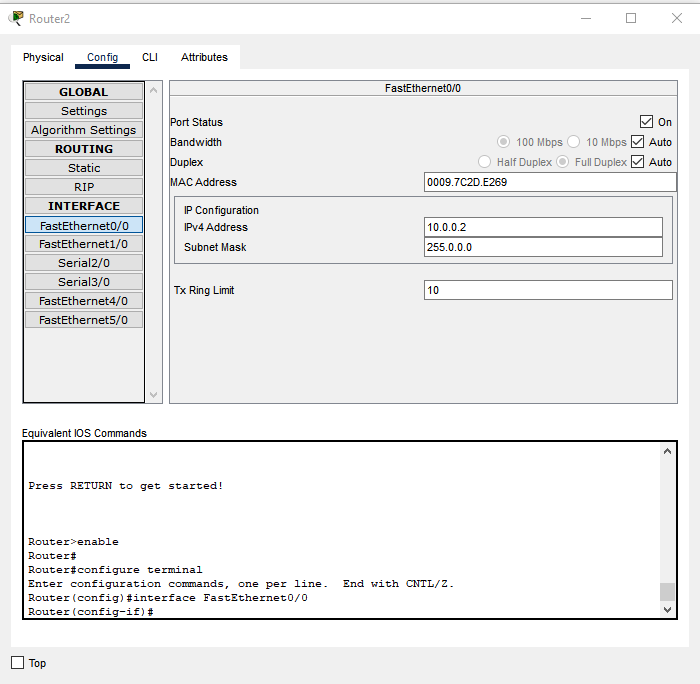
\includegraphics[scale=0.4]{images/1.png}
		\caption{درصد استفاده از هر یک از پروتکل‌ها} 
		\label{s1}
	\end{figure}
	
	
	\item
	مطابق دو شکل \ref{s2} و \ref{s3} درخواست
	\inlineLatin{HTTP GET}
	در زمان
	$1646354879.725804168$
	ارسال شده و پاسخ آن در لحظه
	$1646354880.601833796$
	دریافت شده است. پس فاصله زمانی برابر
	$$1646354880.601833796 - 1646354879.725804168 = 0.876029628 s$$
	است.
	
		\begin{figure}[H]
		\centering
		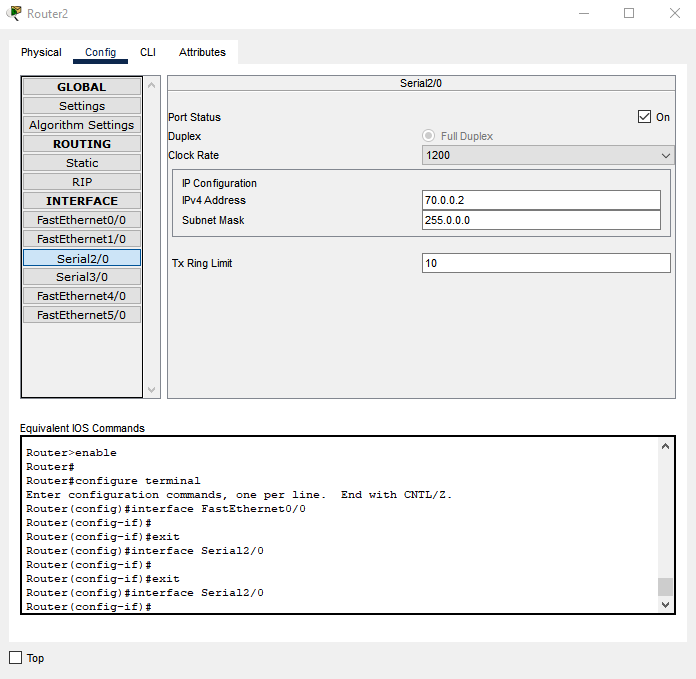
\includegraphics[scale=0.25]{images/2.png}
		\caption{اولین درخواست 
		\inlineLatin{HTTP GET}} 
		\label{s2}
	\end{figure}

	\begin{figure}[H]
	\centering
	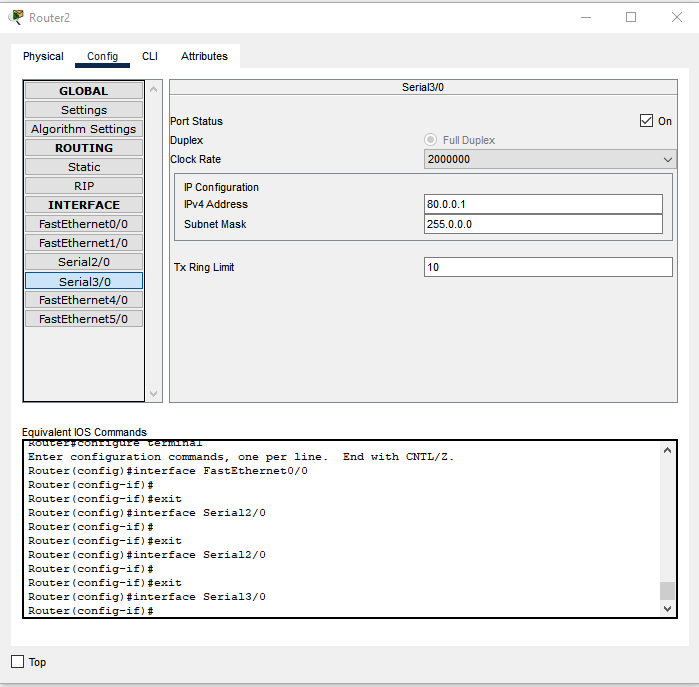
\includegraphics[scale=0.25]{images/3.png}
	\caption{پاسخ
	\inlineLatin{HTTP OK}
نظیر درخواست قبلی} 
	\label{s3}
\end{figure}

برای بدست آوردن شماره ترتیب، از تنظیمات \lr{Preferences} برنامه وایرشارک و قسمت پروتکل \inlineLatin{TCP}، حالت شماره‌گذاری نسبی را غیرفعال می‌کنیم. سپس بر روی اولین درخواست \inlineLatin{HTTP} ارسال شده کلیک راست کرده و گزینه \lr{Follow} و حالت
\inlineLatin{TCP Stream}
را انتخاب می‌کنیم تا بسته‌های \inlineLatin{TCP}
مربوط به آن را بیابیم. با یافتن اولین بسته \inlineLatin{SYN} ارسال شده به جواب می‌رسیم. جواب مطابق شکل \ref{s4} بوده و در این جا شماره ترتیب مطلق برابر
\lr{2296291942}
است.

	\begin{figure}[H]
	\centering
	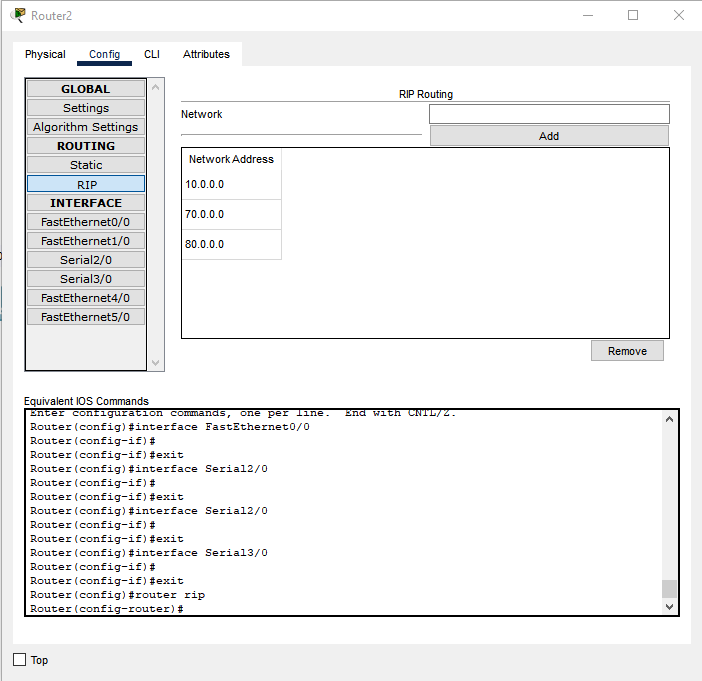
\includegraphics[scale=0.25]{images/4.png}
	\caption{اولین بسته
		\inlineLatin{TCP SYN}
		نظیر درخواست قبلی} 
	\label{s4}
	\end{figure}



\item

مطابق شکل‌های \ref{s5} و \ref{s6} یک کوئری 
\inlineLatin{DNS}
به شکل استاندارد و از نوع
\inlineLatin{A}
به معنی
\lr{Authoritative}
بر بستر پروتکل UDP ارسال شده است و پاسخ آن هم به صورت استاندارد و از نوع
\inlineLatin{A}
بر همین بستر و با آدرس آی‌پی 
\inlineLatin{81.31.186.20}
دریافت شده است.




	\begin{figure}[H]
	\centering
	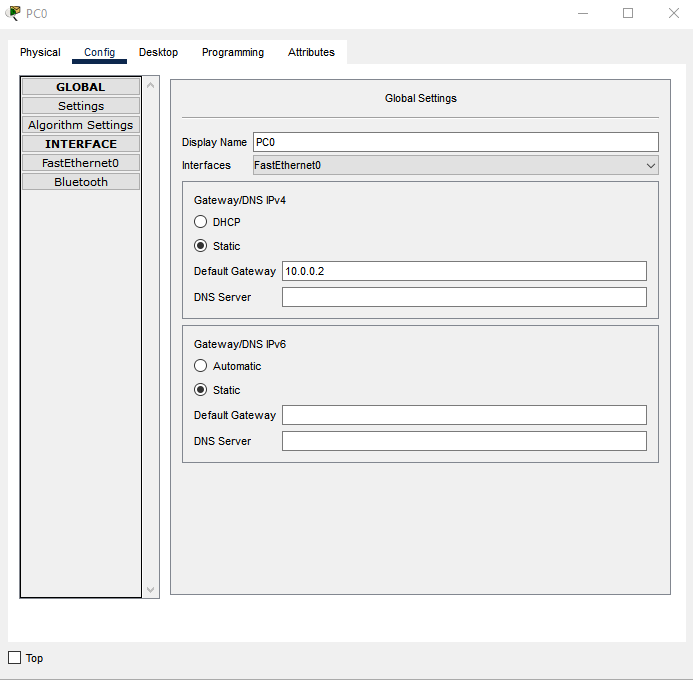
\includegraphics[scale=0.25]{images/5.png}
	\caption{کوئری
	\inlineLatin{DNS}} 
	\label{s5}
	\end{figure}


	\begin{figure}[H]
	\centering
	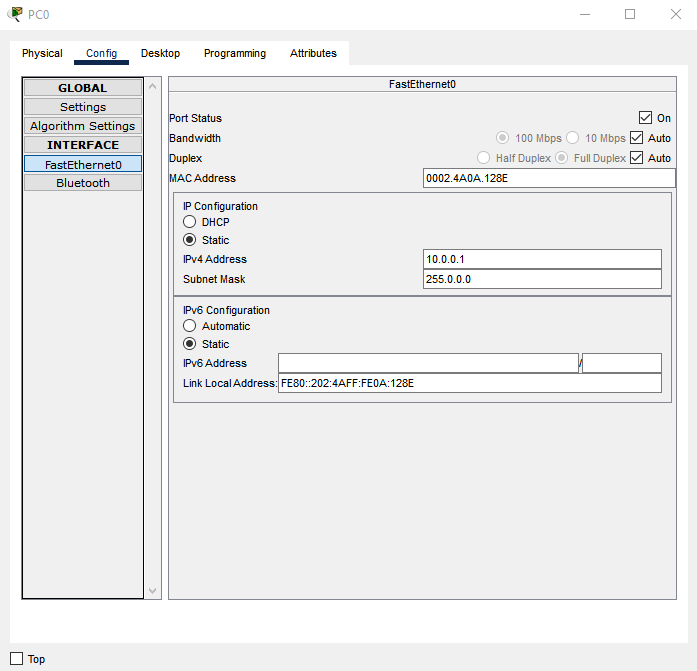
\includegraphics[scale=0.25]{images/6.png}
	\caption{پاسخ
	\inlineLatin{DNS}} 
	\label{s6}
	\end{figure}


\item

مطابق شکل \ref{s7}
برای مشاهده عکس‌ها فیلتر
\inlineLatin{image-jfif}
را روی وایرشارک اعمال می‌کنیم. سپس هر یک از عکس‌های را انتخاب کرده و با کلیک راست روی
\lr{JPEG File Interchangeable Format}
و انتخاب \lr{Export Packet Bytes} عکس‌ها را ذخیره می‌کنیم.

	\begin{figure}[H]
	\centering
	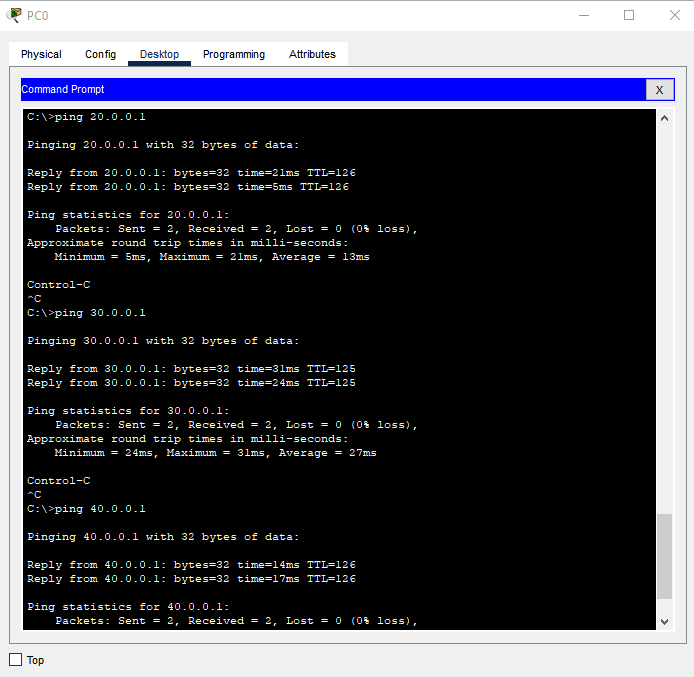
\includegraphics[scale=0.25]{images/7.png}
	\caption{مشاهده شکل‌های دانلود شده از سرور} 
	\label{s7}
\end{figure}

در زیر تعدادی از عکس‌های دانلود شده از سرور که توسط وایرشارک بازیابی شده‌اند را مشاهده می‌کنید.


\begin{figure}[htb]
	\centering
	\begin{subfigure}[b]{\textwidth}
		\centering
		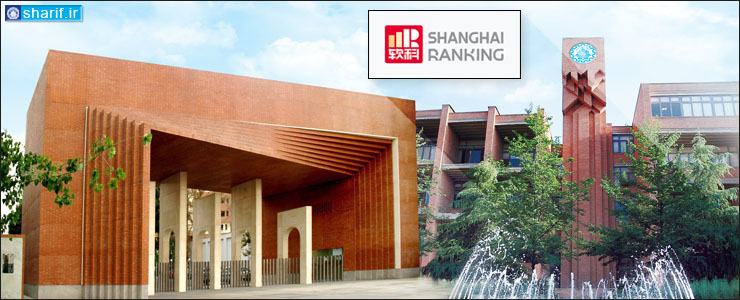
\includegraphics[width=0.2\linewidth]{images/downloaded/im1.jpeg}%
		\hfill
		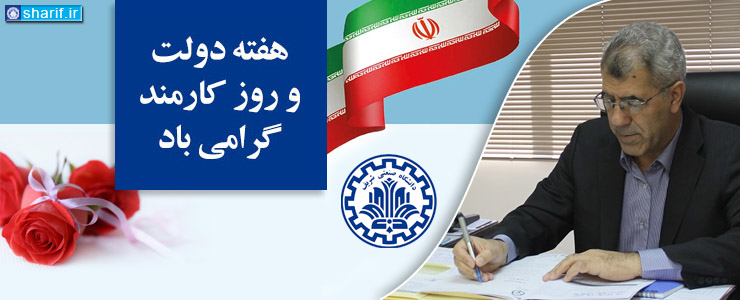
\includegraphics[width=0.2\linewidth]{images/downloaded/im2.jpeg}
		\hfill
		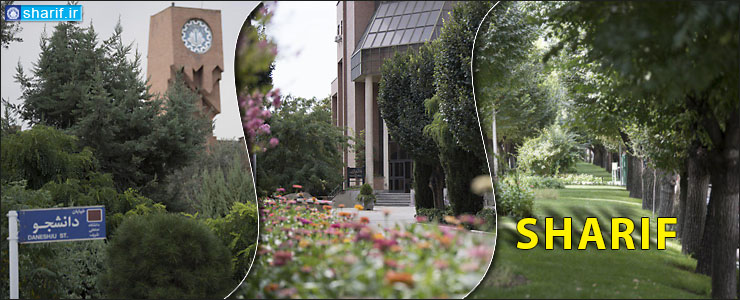
\includegraphics[width=0.2\linewidth]{images/downloaded/im3.jpeg}%
		\hfill
		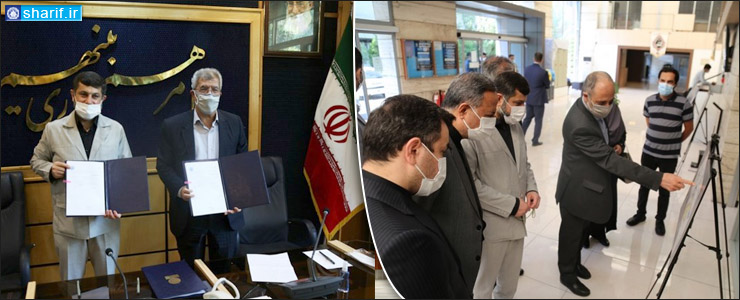
\includegraphics[width=0.2\linewidth]{images/downloaded/im4.jpeg}
	\end{subfigure}
	\vskip\baselineskip
	\begin{subfigure}[b]{\textwidth}
		\centering
		
\includegraphics[width=0.2\linewidth]{images/downloaded/im5.jpeg}%
		\hfill
		
\includegraphics[width=0.2\linewidth]{images/downloaded/im6.jpeg}
		\hfill
		
\includegraphics[width=0.2\linewidth]{images/downloaded/im7.jpeg}%
		\hfill
		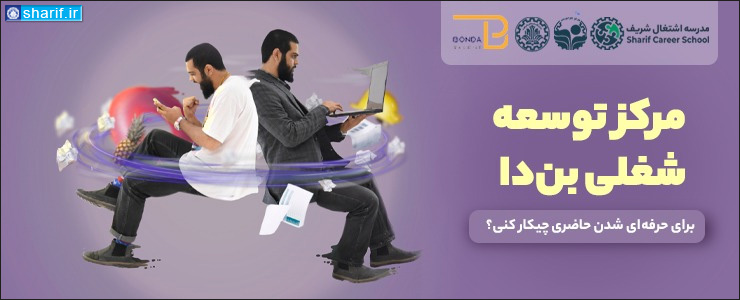
\includegraphics[width=0.2\linewidth]{images/downloaded/im8.jpeg}
	\end{subfigure}
	\vskip\baselineskip
	\begin{subfigure}[b]{\textwidth}
	\centering
	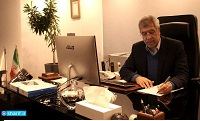
\includegraphics[width=0.2\linewidth]{images/downloaded/im9.jpeg}%
	\hfill
	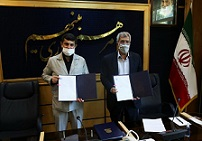
\includegraphics[width=0.2\linewidth]{images/downloaded/im10.jpeg}
	
\end{subfigure}
	\caption{عکس‌های دانلود شده از سرور}
\end{figure}




\end{enumerate}
\newpage

\section{سوالات بخش دوم}

\begin{enumerate}
	
	\item
	مطابق شکل
	\ref{s8}
	و نحوه شروع ارسال پکت‌ها و دریافت آنان،
	آی‌پی مربوط به کلاینت
	\inlineLatin{192.168.0.2}
	و آی‌پی مربوط به سرور
	\inlineLatin{192.168.0.1}
	است.
	
	\begin{figure}[H]
		\centering
		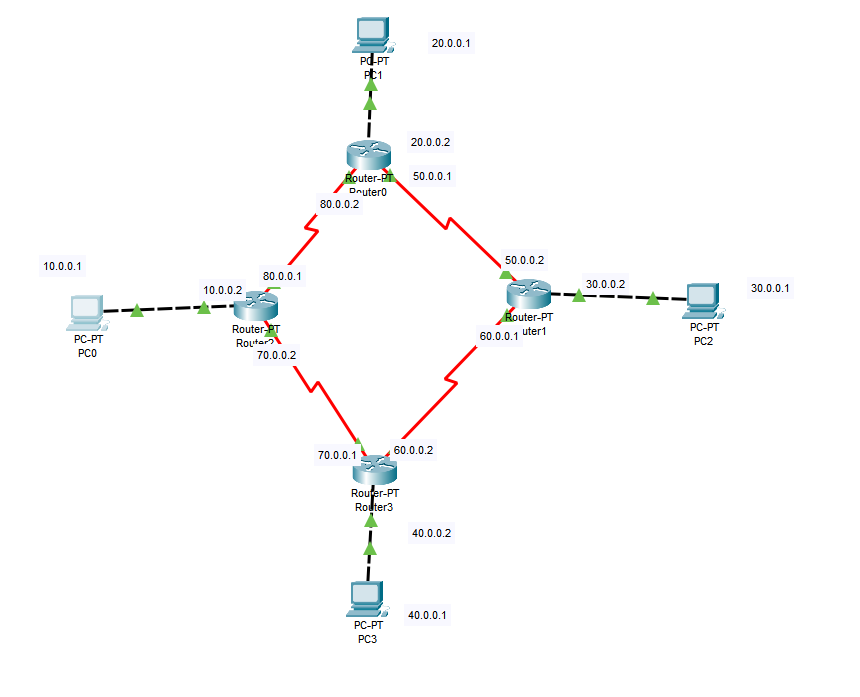
\includegraphics[scale=0.25]{images/8.png}
		\caption{وضعیت کلی پکت‌های ارسالی \inlineLatin{Telnet}} 
		\label{s8}
	\end{figure}
	
	

	برای دو قسمت بعدی، پکت‌های نوع
	\inlineLatin{TELNET}
	را فیلتر کرده، روی اولین مورد کلیک راست کرده و \lr{Follow} و 
	\lr{TCP Stream}
	را انتخاب می‌کنیم. بدین ترتیب کل دستورات و اطلاعات رد و بدل شده را مطابق شکل 
	\ref{s9}
	مشاهده خواهیم کرد.
	
		
	\begin{figure}[H]
		\centering
		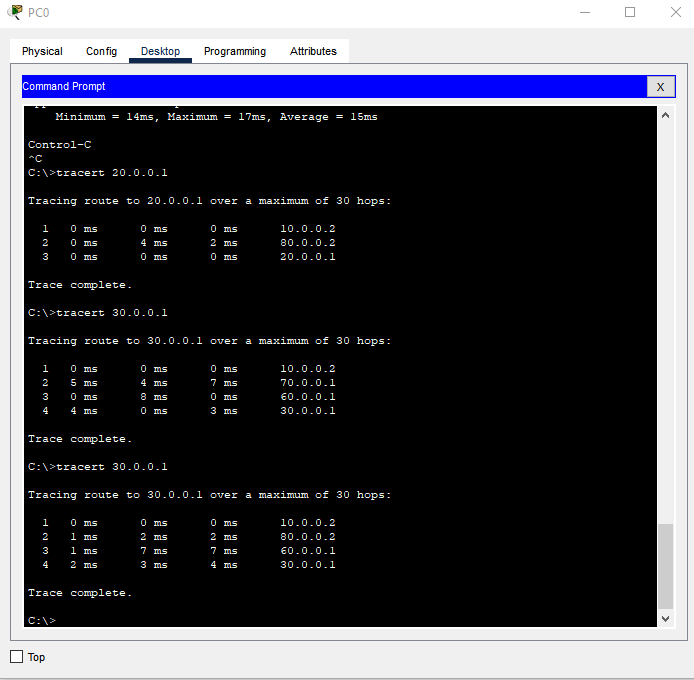
\includegraphics[scale=0.25]{images/9.png}
		\caption{اطلاعات رد و بدل شده در \inlineLatin{Telnet}} 
		\label{s9}
	\end{figure}
	
	\item
	مطابق شکل
	\ref{s9}
	اطلاعات استفاده شده به صورت
	\begin{latin}
		\begin{verbatim}
			
			login: fake
			Password: user
			
		\end{verbatim}
	\end{latin}

	است، پس پسورد استفاده شده
	\inlineLatin{user}
	است.
	
	\item
 	مطابق شکل
	\ref{s9}
	دستورات استفاده شده چهار مورد زیر هستند:
	
	\begin{latin}
		\begin{verbatim}
			
			$ /sbin/ping www.yahoo.com
			$ ls
			$ ls -a
			$ exit
			
		\end{verbatim}
	\end{latin}
	
\end{enumerate}

\newpage

\section{سوالات بخش سوم}

\begin{enumerate}
	\item
مطابق شکل \ref{s10} دستور را در یک سیستم‌عامل لینوکسی و برای سایت 
\inlineLatin{www.digikala.com}
انجام داده‌ایم. از آن جایی که فایل
\inlineLatin{/etc/resolv.conf}
سیستم ما به صورت 

\begin{latin}
	\begin{verbatim}
		nameserver 192.168.1.1
	\end{verbatim}
\end{latin}

تنظیم شده بود، این کوئری برای \inlineLatin{DNS} سرور لوکال یعنی
\inlineLatin{192.168.1.1}
ارسال شده است. در صورتی که دستور را به صورت
\inlineLatin{dig @8.8.8.8 www.digikala.com}
اجرا کنیم، دستور برای \lr{DNS Server} های گوگل به آدرس
\inlineLatin{8.8.8.8}
ارسال می‌شود که این موضوع را در شکل \ref{s11} مشاهده می‌کنید.


	\begin{figure}[H]
	\centering
	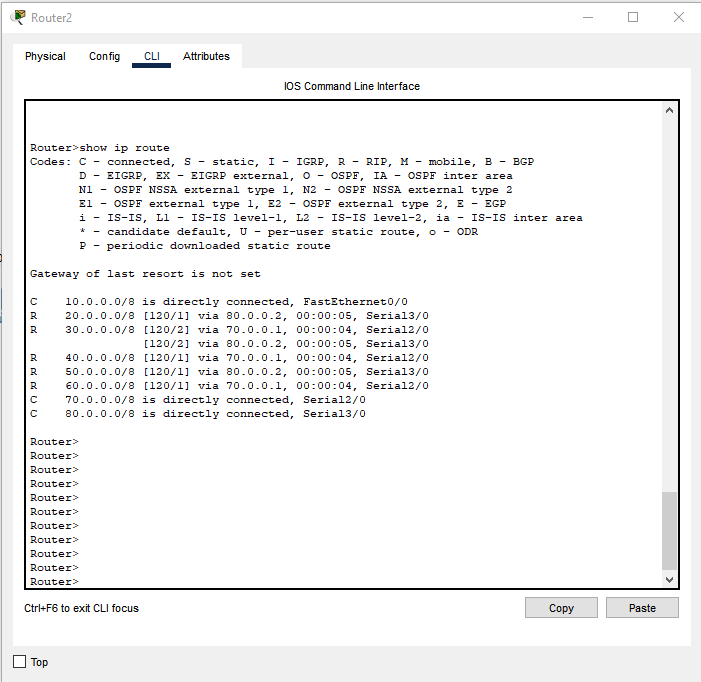
\includegraphics[scale=0.25]{images/10.png}
	\caption{کوئری \inlineLatin{DNS} اجرا شده از طریق دستور
	\inlineLatin{dig www.digikala.com}} 
	\label{s10}
\end{figure}


	\begin{figure}[H]
	\centering
	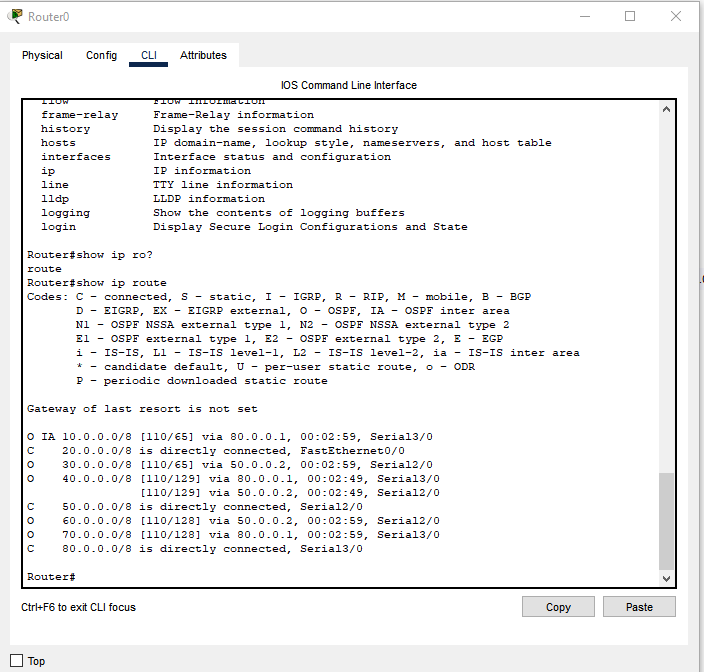
\includegraphics[scale=0.25]{images/12.png}
	\caption{کوئری \inlineLatin{DNS} اجرا شده از طریق دستور
		\inlineLatin{dig @8.8.8.8 www.digikala.com}} 
	\label{s11}
\end{figure}

\item

مطابق شکل‌های \ref{s10} و \ref{s12} که به ترتیب نشان دهنده درخواست و پاسخ هستند، مشاهده می‌کنیم که همان طور که انتظار می‌رود \inlineLatin{DNS} بر بستر \inlineLatin{UDP} ارسال شده و سرآیند‌های رایج آن نظیر پورت مبدا و مقصد را دارد.

علاوه بر آن خود \inlineLatin{DNS} سرآیندهای مخصوص خود را هم دارد. به طور کلی کوئری و پاسخ \inlineLatin{DNS} شامل سرآیند‌های زیر است:

\inlineLatin{Identification}، \inlineLatin{Flags}، \inlineLatin{Number of questions}، \inlineLatin{Number of answers}، \inlineLatin{Number of authority resource records (RRs)} و \inlineLatin{Number of additional RR}
است. در این میان تنها \inlineLatin{flag} نیاز به توضیح اضافی دارد.

در درخواست یعنی شکل
\ref{s10}
مشاهده می‌کنیم که فلگ مربوط به درخواست بودن ست شده است. همچنین مشخص شده که این کوئری استاندارد است. بریده (\lr{Truncate}) نشده است. انجام کوئری به صورت بازگشتی مدنظر است. فلگ \inlineLatin{AD} به معنی
\lr{Authenticate Data}
ست شده است و در فلگ بعدی مشخص شده است که داده‌ای که 
\lr{Authenticate}
نشده قابل قبول نیست. در مورد
\lr{Authenticate Data}
در 
\href{https://datatracker.ietf.org/doc/html/rfc3655}{\textcolor{blue}{\underline{\lr{rfc3655}}}}	 	
توضیحاتی داده شده است.

در پاسخ یعنی شکل
\ref{s12}
در ابتدا مشخص شده که این یک پاسخ است. سپس مشخص شده که از نوع پاسخ استاندارد است. سپس مشخص شده که سرور گفته شده یک
\lr{Authoritative Server}
نیست. پیام بریده نشده است. انجام کوئری به صورت بازگشتی مد نظر قرار گرفته است و امکان پذیر هم بوده است. پاسخ
\lr{Authenticate}
نشده. پاسخ
\lr{Authenticate}
نشده قابل قبول نیست و در نهایت با کد داده شده مشخص شده که پاسخ به اروری برخورد نکرده است.


	\begin{figure}[H]
	\centering
	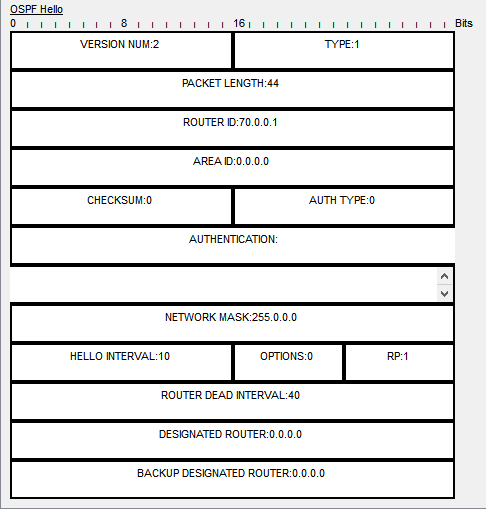
\includegraphics[scale=0.25]{images/11.png}
	\caption{پاسخ دریافت شده \inlineLatin{DNS}  از طریق دستور
		\inlineLatin{dig www.digikala.com}} 
	\label{s12}
\end{figure}
\end{enumerate}

\end{document}



